% JMLR-style preprint generated from the deduplicated FM4PDE ablation outputs.
% The accompanying jmlr2e.sty is the official JMLR style file at commit
% f413f638b407af76074813f8f88a82a7a5a81e9d (retrieved 2026-08-25).
\documentclass[twoside,11pt]{article}

\usepackage[preprint]{jmlr2e}
\usepackage{mathptmx}
\usepackage{amsmath}
\usepackage{booktabs}
\usepackage{tabularx}
\usepackage{array}
\usepackage{multirow}
\usepackage{lastpage}
\usepackage{pgfplots}
\usepackage[section]{placeins}
\usetikzlibrary{patterns}
\pgfplotsset{compat=1.18}
\hypersetup{hidelinks}

\newcolumntype{Y}{>{\raggedright\arraybackslash}X}
\newcommand{\Ebal}{E_{\mathrm{bal}}}
\newcommand{\relA}{\mathrm{RelL2}_a}
\newcommand{\relU}{\mathrm{RelL2}_u}
\newcommand{\Lobsa}{L_{\mathrm{obs},a}}
\newcommand{\Lobsu}{L_{\mathrm{obs},u}}
\newcommand{\Lpde}{L_{\mathrm{PDE}}}
\newcommand{\hsd}{\texttt{hybrid\_s2d}}
\newcommand{\hds}{\texttt{hybrid\_d2s}}

\jmlrheading{0}{2026}{1--\pageref{LastPage}}{8/26}{8/26}{FM4PDE-ABL}{Anonymous Authors}
\ShortHeadings{Ablations for Three PDE Problems}{Anonymous Authors}
\firstpageno{1}

\begin{document}

\title{Sampling, Guidance, and Observation Design in FM4PDE:\
A Systematic Ablation Study on Three PDE Problems}

\author{\name Anonymous Authors \\
        \addr Anonymous affiliation}

\maketitle

\begin{abstract}
We study how guidance composition, loss-evaluation state, sampler phase,
time discretization, observation design, and residual construction affect
physics-guided flow-matching inference on Poisson, Burgers, and non-bounded
Navier--Stokes problems.  After resolving historical reruns, the analysis
contains 274 unique successful configurations: 93 for Poisson, 85 for
Burgers, and 96 for Navier--Stokes.  Observation guidance is the dominant
source of reconstruction accuracy on all three problems, whereas PDE-only
guidance performs similarly to no guidance.  Purely deterministic sampling
is numerically unstable, while a stochastic-to-deterministic schedule can
reduce the reconstruction score by 24\%, 66\%, and 15\% on Poisson,
Burgers, and Navier--Stokes, respectively.  These accuracy gains are not
uniformly physical: the best Poisson and Navier--Stokes schedules increase
the reported PDE residual by factors of 166 and 2.4.  Observation sparsity
also has strongly problem-dependent effects, with a sharp failure below 500
observations for Poisson and below approximately 250--500 observations for
Navier--Stokes, while Burgers degrades more smoothly.  A tighter gradient
clip prevents the Navier--Stokes Hermite residual from producing NaN/Inf,
but 88 of 100 steps remain clipped and reconstruction error is 13.2 times
the endpoint-residual baseline.  The results identify robust default choices
and, equally importantly, configurations that complete without exceptions
but are numerically unusable.
\end{abstract}

\begin{keywords}
  partial differential equations, flow matching, physics guidance,
  inverse problems, ablation study, numerical stability
\end{keywords}

\section{Introduction}
\label{sec:introduction}

Physics-guided generative inference contains several interacting numerical
choices that are not determined by the trained model alone.  Guidance can
be computed from observations, a PDE residual, or both; a loss can be
evaluated at the current noisy state, the next state, or a denoised endpoint;
and the integration path can be stochastic, deterministic, or hybrid.  The
number and placement of observations, the time grid, and the gradient clip
introduce further problem-dependent behavior.  A configuration may therefore
finish successfully while producing a reconstruction many orders of
magnitude worse than a neighboring configuration.

The purpose of this ablation study is to separate these effects under a
common evaluation protocol.  We ask five questions.  First, which guidance
component supplies the information needed for forward, inverse, and joint
reconstruction?  Second, how do the sampler phase and loss-evaluation state
affect stability?  Third, do more time steps or a higher-order integrator
reliably improve accuracy?  Fourth, how sensitive is each PDE to observation
density, placement, and noise?  Fifth, does tighter gradient clipping merely
prevent exceptions, or does it also restore useful Navier--Stokes solutions?

The main empirical conclusion is that there is no single scalar ``best''
configuration.  Observation guidance, endpoint loss evaluation, Euler
integration, and a stochastic component are robust choices across the three
problems.  In contrast, the best hybrid schedule and observation pattern are
problem dependent, and lower reconstruction error can coincide with a larger
PDE residual.  The study is descriptive rather than causal: most individual
configurations use one random seed, while five-seed runs are available only
for the designated stability group.

\section{Experimental Design and Data Processing}
\label{sec:design}

\subsection{Ablation scope}

The experiment varies ten common factors: guidance components, loss state,
sampler phase, time grid, number of steps, integration method, observation
count, observation layout, observation noise, and random seed.  The
Navier--Stokes suite additionally compares three temporal residual modes.
Table~\ref{tab:scope} gives the resulting unique run counts.  Forward runs
score the solution field, inverse runs score the coefficient field, and joint
runs score both fields.  Burgers is represented by one output channel, so its
two stored relative-error fields are identical.

\begin{table}[t]
\caption{Scope of the deduplicated experiment.  Counts refer to unique
analysis-ready runs after historical reruns are removed.}
\label{tab:scope}
\centering
\begin{tabular}{lrrrr}
\toprule
Problem & Forward & Inverse & Joint & Total \\
\midrule
Poisson & 4 & 4 & 85 & 93 \\
Burgers & 0 & 0 & 85 & 85 \\
Non-bounded Navier--Stokes & 4 & 4 & 88 & 96 \\
\midrule
Total & 8 & 8 & 258 & 274 \\
\bottomrule
\end{tabular}
\end{table}

The reference joint configuration uses observation and PDE guidance, an
endpoint loss, stochastic sampling, a uniform 100-step grid, Euler updates,
500 per-sample random observations, and zero observation noise.  Ablation
groups modify one design dimension around this reference.  Identical anchor
configurations intentionally recur in different groups; they are retained
because they provide within-group comparisons and are not historical
duplicates.

\subsection{Run identity and removal of historical duplicates}
\label{sec:dedup}

The historical aggregate contains 355 final-metric records.  We define run
identity by the composite key
\[
  (\text{PDE},\ \text{task},\ \texttt{ablation\_name}).
\]
Within each identity, we retain the most recent run satisfying
\texttt{status=ok}, a non-error PDE evaluation status, and finite values for
\(\relA\), \(\relU\), and \(\Lpde\).  This procedure produces 274 unique
records and excludes 81 superseded records.  All 81 exclusions are older
Navier--Stokes joint runs with \texttt{clip\_threshold=}\(10^{10}\); Poisson
and Burgers have no historical rerun duplicates.  The historical file remains
unchanged for auditability, while the paper uses only
\path{summary_latest_unique.csv}.  The complete exclusions and their selected
replacements are recorded in \path{summary_excluded_runs.csv}.

The selected records all pass status, step-count, sample-count, and finite
metric checks.  Resolved clipping thresholds are 50 for all Burgers runs;
\(10^{10}\) for Poisson joint/forward and Navier--Stokes forward; 50 for
Poisson and Navier--Stokes inverse runs; and \(10^4\) for Navier--Stokes
joint runs.

\subsection{Metrics and comparison rules}
\label{sec:metrics}

Every reported configuration contains five primitive metrics: coefficient-field
relative error \(\relA\), solution-field relative error \(\relU\), coefficient
observation loss \(\Lobsa\), solution observation loss \(\Lobsu\), and PDE loss
\(\Lpde\).  The relative errors are mean per-sample relative \(L_2\) errors;
the observation losses are the final unweighted masked MSE values against the
actual observations, including configured observation noise.  Clean-target
observation losses remain available in the aggregate files as diagnostics.

For ranking joint Poisson and Navier--Stokes runs only, we define the balanced
reconstruction index
\begin{equation}
  \Ebal = \frac{\relA + \relU}{2}.
  \label{eq:balanced}
\end{equation}
For forward and inverse tasks, the target score is \(\relU\) and \(\relA\),
respectively.  For Burgers, the target score is the single-channel relative
error.  Equal weighting in Equation~\ref{eq:balanced} is an analysis convention
rather than a new training objective, and the index never replaces the
separately reported \(a\)- and \(u\)-field errors.  The complete one-row-per-run
reporting view is \path{ablation_report_metrics.csv}; its stable metric columns
are \texttt{rel\_l2\_a}, \texttt{rel\_l2\_u}, \texttt{L\_obs\_a},
\texttt{L\_obs\_u}, and \texttt{L\_pde}.

The reported \(\Lpde\) is used as a physical-consistency diagnostic only
when the residual definition is unchanged.  It must not be compared directly
across endpoint secant, Hermite bridge, and near-endpoint temporal modes,
which use different residual channels and normalizations.  Unless a result is
drawn from the five-seed stability group, values represent one run with batch
size one and should be interpreted as effect-size diagnostics rather than
formal statistical estimates.

\section{Observation Guidance Supplies the Reconstruction Signal}
\label{sec:guidance}

Across every problem and task, observation guidance reduces the target error
by approximately one to two orders of magnitude relative to no guidance.
Table~\ref{tab:guidance} reports the complete guidance-component sweep.  PDE
guidance alone is nearly indistinguishable from no guidance.  Adding the PDE
term to observation guidance produces only a small forward-task improvement
for Navier--Stokes and no consistent improvement elsewhere.

\begin{table}[t]
\caption{Complete primitive metrics for the guidance-component ablation.
NS denotes non-bounded Navier--Stokes.  Observation losses are reported for
both fields even when the task gate activates only one of them.}
\label{tab:guidance}
\centering
\scriptsize
\resizebox{\textwidth}{!}{%
\begin{tabular}{lllrrrrr}
\toprule
Problem & Task & Guidance & \(\relA\) & \(\relU\) & \(\Lobsa\) & \(\Lobsu\) & \(\Lpde\) \\
\midrule
Poisson & Forward & No guide & 0.706328 & 0.636149 & 0.0475036 & $8.30383\!\times\!10^{-6}$ & 0.00501552 \\
Poisson & Forward & PDE only & 0.706371 & 0.636293 & 0.0475095 & $8.30763\!\times\!10^{-6}$ & 0.00501407 \\
Poisson & Forward & Obs. only & 0.104347 & 0.0567385 & 0.000759209 & $7.49590\!\times\!10^{-8}$ & 0.00493408 \\
Poisson & Forward & Obs.+PDE & 0.104354 & 0.0567902 & 0.000759369 & $7.50893\!\times\!10^{-8}$ & 0.00492117 \\
Poisson & Inverse & No guide & 0.706328 & 0.636149 & 0.0475036 & $8.30383\!\times\!10^{-6}$ & 0.00501552 \\
Poisson & Inverse & PDE only & 0.706474 & 0.636608 & 0.0475234 & $8.31597\!\times\!10^{-6}$ & 0.00499225 \\
Poisson & Inverse & Obs. only & 0.184290 & 0.0400967 & 0.00369552 & $3.34923\!\times\!10^{-8}$ & 0.00495474 \\
Poisson & Inverse & Obs.+PDE & 0.184284 & 0.0400938 & 0.00369519 & $3.34877\!\times\!10^{-8}$ & 0.00493661 \\
Poisson & Joint & No guide & 0.706328 & 0.636149 & 0.0475036 & $8.30383\!\times\!10^{-6}$ & 0.00501552 \\
Poisson & Joint & PDE only & 0.706365 & 0.636290 & 0.0475089 & $8.30756\!\times\!10^{-6}$ & 0.00501193 \\
Poisson & Joint & Obs. only & 0.0987497 & 0.0335385 & 0.000674767 & $2.47046\!\times\!10^{-8}$ & 0.00486790 \\
Poisson & Joint & Obs.+PDE & 0.0987495 & 0.0335390 & 0.000674772 & $2.47065\!\times\!10^{-8}$ & 0.00485743 \\
\midrule
Burgers & Joint & No guide & 1.08051 & 1.08051 & 0.109369 & 0.106683 & 0.000746940 \\
Burgers & Joint & PDE only & 1.06139 & 1.06139 & 0.105655 & 0.103229 & 0.000643136 \\
Burgers & Joint & Obs. only & 0.0161125 & 0.0161125 & $2.20532\!\times\!10^{-5}$ & $2.04047\!\times\!10^{-5}$ & 0.00304960 \\
Burgers & Joint & Obs.+PDE & 0.0160872 & 0.0160872 & $2.19834\!\times\!10^{-5}$ & $2.03668\!\times\!10^{-5}$ & 0.00298843 \\
\midrule
NS & Forward & No guide & 1.20948 & 0.997277 & 0.0549511 & 0.0441466 & 0.00243790 \\
NS & Forward & PDE only & 1.20948 & 0.997271 & 0.0549515 & 0.0441461 & 0.00243838 \\
NS & Forward & Obs. only & 0.214954 & 0.124017 & 0.00138949 & 0.000725228 & 0.00276624 \\
NS & Forward & Obs.+PDE & 0.213913 & 0.122684 & 0.00138016 & 0.000716983 & 0.00271786 \\
NS & Inverse & No guide & 1.20948 & 0.997277 & 0.0549511 & 0.0441466 & 0.00243790 \\
NS & Inverse & PDE only & 1.20952 & 0.997295 & 0.0549539 & 0.0441498 & 0.00243765 \\
NS & Inverse & Obs. only & 0.342449 & 0.206961 & 0.00473021 & 0.00162207 & 0.00273852 \\
NS & Inverse & Obs.+PDE & 0.346227 & 0.209956 & 0.00484030 & 0.00166886 & 0.00273813 \\
NS & Joint & No guide & 1.20948 & 0.997277 & 0.0549511 & 0.0441466 & 0.00243790 \\
NS & Joint & PDE only & 1.20943 & 0.997223 & 0.0549473 & 0.0441453 & 0.00243845 \\
NS & Joint & Obs. only & 0.199914 & 0.115232 & 0.00111870 & 0.000584215 & 0.00277407 \\
NS & Joint & Obs.+PDE & 0.199993 & 0.115158 & 0.00112182 & 0.000581448 & 0.00277131 \\
\bottomrule
\end{tabular}
}
\end{table}

The result does not imply that the PDE term is intrinsically useless.  It
shows that, under the tested weights and residual definitions, the observation
loss already provides nearly all of the reconstruction signal.  Moreover, a
small PDE residual alone is not sufficient for identification: Burgers
PDE-only guidance obtains \(\Lpde=6.43\times 10^{-4}\), smaller than the
observation-guided baseline, while its reconstruction error is 1.061 rather
than 0.016.  The PDE admits many low-residual fields that are not the target
field; observations select among those fields.

\section{Stochastic-to-Deterministic Sampling Improves Accuracy but Can Harm the Residual}
\label{sec:sampling}

Endpoint loss evaluation with a stochastic component is the only setting
that is reliable across all three problems.  Evaluating guidance at
\texttt{xt} or \texttt{x\_next} raises the stochastic target score from
0.066 to 0.346/0.257 on Poisson, from 0.016 to 0.629/0.481 on Burgers, and
from 0.158 to 0.359/1.153 on Navier--Stokes.  Replacing stochastic sampling
with a deterministic endpoint update produces scores of
\(2.56\times10^4\), \(2.63\times10^3\), and \(1.36\times10^5\),
respectively.

Hybrid schedules can outperform the stochastic reference, but their optimal
switch points differ by problem.  Table~\ref{tab:sampling-best} and
Figure~\ref{fig:sampling-normalized} compare the best sampler-phase and
time-grid variants with the reference joint score.  Burgers benefits most:
\hsd{} with switch ratio 0.2 reduces the error by 66.3\%.  Poisson also
improves, but its best phase setting multiplies \(\Lpde\) by 166.
Navier--Stokes obtains its best reconstruction from cosine + \hsd{}, with a
32.0\% score reduction and a 13.9-fold residual increase.

\begin{table}[t]
\caption{Primitive metrics for the stochastic reference and the settings
selected by the sampler-phase and time-grid ranking indices.}
\label{tab:sampling-best}
\centering
\scriptsize
\resizebox{\textwidth}{!}{%
\begin{tabular}{lllrrrrr}
\toprule
Problem & Source & Setting & \(\relA\) & \(\relU\) & \(\Lobsa\) & \(\Lobsu\) & \(\Lpde\) \\
\midrule
Poisson & Reference & Stochastic & 0.0987495 & 0.0335390 & 0.000674772 & $2.47065\!\times\!10^{-8}$ & 0.00485743 \\
Poisson & Phase & \hsd{}, 0.2 & 0.0858454 & 0.0151030 & 0.000580406 & $4.34068\!\times\!10^{-9}$ & 0.804162 \\
Poisson & Grid & Cosine + \hsd{} & 0.0895861 & 0.0194788 & 0.000569167 & $8.42302\!\times\!10^{-9}$ & 0.0271510 \\
\midrule
Burgers & Reference & Stochastic & 0.0160872 & 0.0160872 & $2.19834\!\times\!10^{-5}$ & $2.03668\!\times\!10^{-5}$ & 0.00298843 \\
Burgers & Phase & \hsd{}, 0.2 & 0.00541692 & 0.00541692 & $2.81017\!\times\!10^{-6}$ & $2.75459\!\times\!10^{-6}$ & 0.00667524 \\
Burgers & Grid & Cosine + \hsd{} & 0.00552473 & 0.00552473 & $3.12696\!\times\!10^{-6}$ & $2.08008\!\times\!10^{-6}$ & 0.00273157 \\
\midrule
Navier--Stokes & Reference & Stochastic & 0.199993 & 0.115158 & 0.00112182 & 0.000581448 & 0.00277131 \\
Navier--Stokes & Phase & \hsd{}, 0.5 & 0.183344 & 0.0850448 & 0.000875568 & 0.000297114 & 0.00669611 \\
Navier--Stokes & Grid & Cosine + \hsd{} & 0.156057 & 0.0581717 & 0.000575255 & 0.000126354 & 0.0385353 \\
\bottomrule
\end{tabular}
}
\end{table}

\begin{figure}[t]
\centering
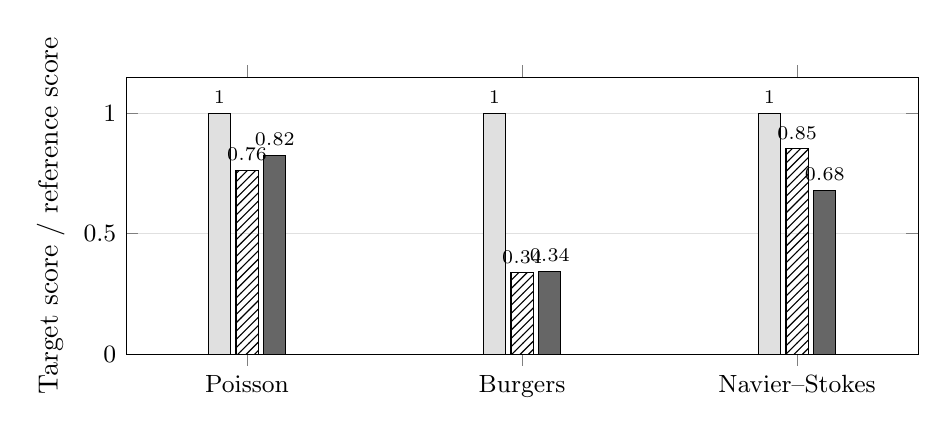
\begin{tikzpicture}
\begin{axis}[
  width=0.96\linewidth,
  height=5.1cm,
  ybar,
  bar width=8pt,
  ymin=0,
  ymax=1.15,
  ylabel={Target score / reference score},
  symbolic x coords={Poisson,Burgers,Navier--Stokes},
  xtick=data,
  enlarge x limits=0.22,
  ymajorgrids=true,
  grid style={black!12},
  nodes near coords,
  every node near coord/.append style={font=\scriptsize},
  tick label style={font=\small},
]
\addplot[draw=black,fill=black!12] coordinates
  {(Poisson,1.000) (Burgers,1.000) (Navier--Stokes,1.000)};
\addplot[draw=black,fill=white,pattern=north east lines] coordinates
  {(Poisson,0.763) (Burgers,0.337) (Navier--Stokes,0.852)};
\addplot[draw=black,fill=black!60] coordinates
  {(Poisson,0.824) (Burgers,0.343) (Navier--Stokes,0.680)};
\end{axis}
\end{tikzpicture}
\caption{Best reconstruction scores normalized by the joint stochastic
reference for each PDE.  Values below one indicate an accuracy improvement.
Within each PDE, the bars from left to right show the reference, best phase
sweep, and best grid sweep.
The figure is a ranking visualization only; Table~\ref{tab:sampling-best}
reports both field errors and all loss components separately.}
\label{fig:sampling-normalized}
\end{figure}

The common mechanism is consistent with early stochastic exploration followed
by late deterministic refinement.  Beginning deterministically and switching
to stochastic sampling is much less reliable: \hds{} with switch ratio 0.8
produces errors of 3334 on Poisson, 343 on Burgers, and 17744 on
Navier--Stokes.  The exact switch point is nevertheless problem specific,
which argues against treating a hybrid schedule as a universal default.

\section{More Steps and Midpoint Integration Do Not Give Universal Gains}
\label{sec:discretization}

Step-count effects differ across the PDEs.  In the step sweep, Poisson reaches
its lowest score at 2000 stochastic steps (0.05953), compared with 0.06614 at
100 steps, but wall-clock time grows from approximately 9 to 179 seconds.
Burgers reaches its stochastic minimum at 1000 steps (0.00815) and slightly
regresses at 2000 steps (0.00868); the 50-step \hsd{} result is already
0.00992.  Navier--Stokes is qualitatively different: \hsd{} is best at 100
steps (0.13453), and additional steps do not improve it; stochastic sampling
also worsens beyond 100 steps.  Consequently, the number of steps is a
problem- and schedule-dependent regularization choice rather than a monotone
accuracy control.

Midpoint integration increases 100-step runtime by factors of 1.50 on
Poisson, 1.50 on Burgers, and 1.66 on Navier--Stokes.  Its reconstruction
changes are small and inconsistent.  For example, midpoint slightly improves
Navier--Stokes \hsd{} from 0.13336 to 0.13279, but raises \(\Lpde\) from
0.00689 to 0.01066.  The change is smaller than the five-seed variability and
does not justify the additional compute as a default.  Euler is therefore the
more defensible baseline.

\section{Observation Requirements Are Strongly Problem Dependent}
\label{sec:observations}

Observation density is the largest source of cross-problem heterogeneity.
Figure~\ref{fig:sensor-sparsity} normalizes each sparsity result by its
500-observation score.  Poisson shows a sharp transition: 250 observations
are 12.9 times worse than 500, and 50 observations are 100 times worse.
Navier--Stokes is also unstable at 50--100 observations but is within 17\% of
the 500-observation result at 250.  Burgers degrades smoothly; 50 observations
approximately double the error rather than causing an order-of-magnitude
failure.  Increasing from 500 to 1000 observations produces no material gain
for any problem.

\begin{figure}[t]
\centering
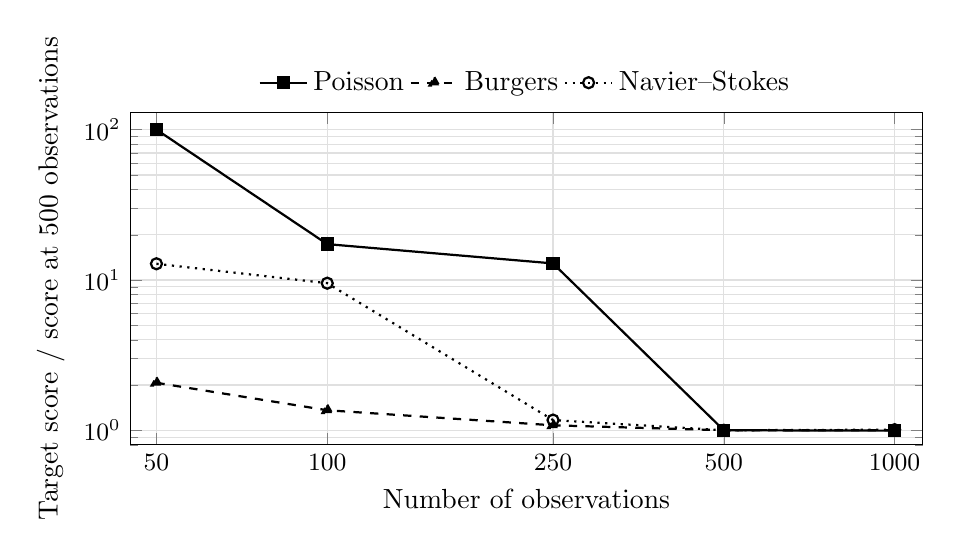
\begin{tikzpicture}
\begin{axis}[
  width=0.96\linewidth,
  height=5.8cm,
  xmode=log,
  ymode=log,
  log basis x=10,
  log basis y=10,
  xmin=45,
  xmax=1120,
  ymin=0.8,
  ymax=130,
  xtick={50,100,250,500,1000},
  xticklabels={50,100,250,500,1000},
  xlabel={Number of observations},
  ylabel={Target score / score at 500 observations},
  legend style={at={(0.5,1.02)},anchor=south,legend columns=3,draw=none},
  grid=both,
  grid style={black!12},
  tick label style={font=\small},
]
\addplot[black,mark=square*,thick] coordinates
  {(50,100.190) (100,17.332) (250,12.898) (500,1.000) (1000,0.994)};
\addplot[black,dashed,mark=triangle*,thick] coordinates
  {(50,2.070) (100,1.359) (250,1.079) (500,1.000) (1000,1.000)};
\addplot[black,dotted,mark=o,mark options={solid},thick] coordinates
  {(50,12.827) (100,9.525) (250,1.169) (500,1.000) (1000,1.009)};
\legend{Poisson,Burgers,Navier--Stokes}
\end{axis}
\end{tikzpicture}
\caption{Sensitivity to observation sparsity.  Ratios are computed within
each PDE relative to its 500-observation run; both axes are logarithmic.
Line style and marker shape duplicate the series distinction for grayscale
readability.}
\label{fig:sensor-sparsity}
\end{figure}

Placement is similarly problem dependent.  Random and per-sample random masks
are best for Poisson (score 0.06614), whereas a fixed mask is poor (1.150).
Burgers obtains a promising fixed-mask score of 0.00592, compared with 0.01609
for per-sample random masks, but this is a single-mask result and may reflect a
favorable placement.  Navier--Stokes prefers a grid (0.15542); fixed and
sensor-column layouts degrade to 0.854 and 0.477.  These results support
problem-specific mask design rather than a single universal sensor policy.

Noise sensitivity also differs.  At 10\% noise, the target score changes by
+4.4\% for Poisson, +63.9\% for Burgers, and $-0.2\%$ for Navier--Stokes
relative to the corresponding zero-noise run.  The small apparent
Navier--Stokes improvement is below seed variation and should be interpreted
as no detectable degradation, not as a beneficial effect of noise.

\section{Stability Checks Separate Runtime Success from Numerical Success}
\label{sec:stability}

Five-seed results quantify baseline variability (Table~\ref{tab:stability}).
Navier--Stokes is the most repeatable in reconstruction score, with a 2.05\%
coefficient of variation.  Burgers has 15.1\% relative variability.  Poisson's
balanced score varies by 12.5\%, while its solution error and PDE residual
have coefficients of variation of 37.1\% and 49.0\%, respectively.  Small
single-run differences---including most observation-only versus
observation+PDE differences---are therefore not statistically distinguishable
under the available replication.

\begin{table}[t]
\caption{Five-seed stability of the reference configuration.  Each cell is
mean $\pm$ sample standard deviation; no balanced score replaces the two
field-level errors.}
\label{tab:stability}
\centering
\scriptsize
\resizebox{\textwidth}{!}{%
\begin{tabular}{lrrrrr}
\toprule
Problem & \(\relA\) & \(\relU\) & \(\Lobsa\) & \(\Lobsu\) & \(\Lpde\) \\
\midrule
Poisson & $0.10555\!\pm\!0.00598$ & $0.03890\!\pm\!0.01442$ & $7.80\!\times\!10^{-4}\!\pm\!1.10\!\times\!10^{-4}$ & $3.45\!\times\!10^{-8}\!\pm\!2.72\!\times\!10^{-8}$ & $0.003744\!\pm\!0.001836$ \\
Burgers & $0.01458\!\pm\!0.00220$ & $0.01458\!\pm\!0.00220$ & $1.89\!\times\!10^{-5}\!\pm\!5.63\!\times\!10^{-6}$ & $1.51\!\times\!10^{-5}\!\pm\!3.77\!\times\!10^{-6}$ & $0.003354\!\pm\!0.000523$ \\
Navier--Stokes & $0.19816\!\pm\!0.00415$ & $0.11696\!\pm\!0.00357$ & $0.001082\!\pm\!0.000096$ & $0.000577\!\pm\!0.000014$ & $0.003056\!\pm\!0.000199$ \\
\bottomrule
\end{tabular}
}
\end{table}

Every one of the 274 selected records has finite final metrics, but 57
configurations have a target score of at least 10: 20 Poisson, 17 Burgers,
and 20 Navier--Stokes runs.  These cases are concentrated in deterministic
sampling, late \hds{} switches, and incompatible time grids.  We classify
them as numerical divergence despite \texttt{status=ok}.  This distinction is
important: exception-free execution is a software property, whereas a useful
reconstruction is a numerical property.

The Navier--Stokes Hermite residual illustrates a third failure mode.  With a
clip threshold of \(10^{10}\), the original run records five steps and
then terminates because the PDE loss contains NaN/Inf.  Repeating the run at
\(10^4\) completes all 100 steps, but clipping is active for 88 steps and the
minimum gradient scale is 0.054.  Its balanced score is 2.078, compared with
0.158 for endpoint secant, a 13.2-fold degradation.  Tighter clipping thus
solves the runtime exception but not the underlying stiffness or objective
mis-scaling.

\section{Discussion and Practical Recommendations}
\label{sec:discussion}

The three PDE suites support four general conclusions.

\paragraph{Observations identify the solution; the tested PDE term mainly
regularizes it.}
PDE-only guidance does not recover the target even when its residual is small.
This behavior is expected when many fields approximately satisfy the operator
but only a subset agrees with the observed coefficient or solution.  The
present weights make the PDE term a weak discriminator after observations are
available.  A stronger claim would require re-tuning the PDE coefficient and
replicating the comparison across seeds.

\paragraph{Stochasticity is a stability mechanism.}
Pure deterministic sampling is consistently catastrophic.  A late
deterministic phase can improve accuracy, but only after stochastic sampling
has kept the trajectory in a stable region.  We recommend endpoint loss,
Euler integration, and a stochastic reference as the default.  A
problem-specific \hsd{} schedule should be treated as a tuned alternative:
ratio 0.2 is promising for Poisson and Burgers, while ratio 0.5 with a cosine
grid is the strongest Navier--Stokes accuracy candidate.

\paragraph{Accuracy and physical residual form a Pareto problem.}
The best reconstruction setting is not always the setting with the smallest
\(\Lpde\).  Poisson and Navier--Stokes gain accuracy at a substantial residual
cost, while Burgers cosine + \hsd{} improves both quantities relative to the
reference.  Future model selection should report a two-objective Pareto front
rather than rank configurations by reconstruction error alone.

\paragraph{Observation policy must follow the operator.}
For the tested resolution and guidance weights, 500 observations are a safe
cross-problem default.  Poisson should not be reduced below this value without
retuning; Navier--Stokes may tolerate 250 but is unstable at 100; Burgers is
more tolerant but more sensitive to noise.  Fixed or structured masks require
multiple-mask replication before they can be recommended.

On current evidence, we advise against pure deterministic sampling, large
\hds{} switch ratios, and the present Hermite residual.  Midpoint integration
does not offer a favorable accuracy--cost tradeoff.  The strongest candidates
for a confirmatory study are Burgers \hsd{} at ratio 0.2 and
Navier--Stokes cosine + \hsd{} at ratio 0.5, each evaluated with at least five
seeds and with reconstruction and physical residual reported jointly.

\section{Limitations}
\label{sec:limitations}

This study has five main limitations.  First, most configurations contain one
sample and one seed; only the stability group has five independent seeds.
Second, the study is one-factor-at-a-time rather than fully factorial, so the
best settings from different groups cannot be assumed to combine additively.
Third, selecting the best run among many single-seed alternatives introduces
selection bias and multiple-comparison risk.  Fourth, the equal-weight
balanced score may not reflect application-specific costs for coefficient and
solution errors.  Fifth, \(\Lpde\) is residual-definition dependent and does
not measure all forms of physical plausibility.

There is also a reproducibility hazard in the current repository state.  The
selected Navier--Stokes joint runs resolve to a clip threshold of \(10^4\),
but \path{configs/main/both/nsnonbounded.yaml} still contains \(10^{10}\).
The stable threshold should be committed to a canonical configuration or
passed through an explicit, recorded override before the sweep is rerun.

\section{Conclusion}
\label{sec:conclusion}

The deduplicated 274-run study shows that observation guidance, endpoint loss
evaluation, and stochastic sampling are the most transferable design choices
across Poisson, Burgers, and non-bounded Navier--Stokes problems.  Hybrid
stochastic-to-deterministic sampling can improve reconstruction substantially,
but the optimal switch is problem dependent and can increase the PDE residual.
More steps and higher-order integration are not uniformly beneficial, and
observation density has distinct thresholds across operators.  Finally,
gradient clipping should be interpreted as a safety mechanism rather than a
guarantee of useful solutions: it prevents the Hermite residual from crashing
but leaves the method heavily clipped and inaccurate.  These findings narrow
the stable design space and define the multi-seed, multi-objective experiments
needed for a defensible final configuration.

\appendix

\section{Complete Group-Level Summary}
\label{app:complete}

The complete group-level report is emitted as
\path{ablation_report_metrics.csv}.  It contains one selected row for every
\((\mathrm{PDE},\mathrm{task},\texttt{ablation\_name})\) identity, including
all 274 currently completed configurations.  Unlike the previous appendix,
it does not collapse \(\relA\) and \(\relU\) into a target score and does not
omit the observation losses.  Table~\ref{tab:report-contract} defines its
stable metric contract; configuration columns and source paths accompany
these values in the CSV.

\begin{table}[t]
\caption{Required columns in the complete ablation reporting view.}
\label{tab:report-contract}
\centering
\begin{tabular}{lll}
\toprule
CSV column & Symbol & Definition \\
\midrule
\texttt{rel\_l2\_a} & \(\relA\) & Coefficient-field relative \(L_2\) error \\
\texttt{rel\_l2\_u} & \(\relU\) & Solution-field relative \(L_2\) error \\
\texttt{L\_obs\_a} & \(\Lobsa\) & Final masked observation MSE for \(a\) \\
\texttt{L\_obs\_u} & \(\Lobsu\) & Final masked observation MSE for \(u\) \\
\texttt{L\_pde} & \(\Lpde\) & Final evaluation PDE loss \\
\bottomrule
\end{tabular}
\end{table}

For repeated configurations, \path{summary_latest_run_seed_grouped.csv}
reports mean, sample standard deviation, standard error, 95\% interval
half-width, median, p90, minimum, and maximum separately for all five fields.

\section{Data Quality and Reproducibility Artifacts}
\label{app:artifacts}

The analysis is backed by the following files in \path{outputs/ablations}:
\begin{itemize}
  \item \path{summary_all_raw.csv}: all 355 historical final records;
  \item \path{summary_latest_unique.csv}: the 274-record analysis snapshot;
  \item Complete reporting view with separate \(\relA\), \(\relU\),
        \(\Lobsa\), \(\Lobsu\), and \(\Lpde\):
        \path{ablation_report_metrics.csv};
  \item \path{summary_excluded_runs.csv}: the 81 superseded records and their replacements;
  \item \path{summary_latest_run_seed_grouped.csv}: grouped run-level
        statistics for the same five primitive metrics;
  \item \path{metrics_per_sample_latest_unique.csv}: per-sample current records; and
  \item \path{curves_latest_grouped.csv}: step-level curves restricted to selected runs.
\end{itemize}

The supporting code is also auditable:
\begin{itemize}
  \item \path{sampling/aggregate.py} implements the latest-snapshot selector; and
  \item \path{tests/test_aggregate_results.py} verifies that historical rows are preserved while superseded rows are excluded from the current snapshot.
\end{itemize}
The selector uses a deterministic recency tie-break and emits an explicit
exclusion reason for every discarded final record.

\end{document}
